% !TEX TS-program = pdflatex
\documentclass[11pt]{article}

% -------------------- Packages --------------------
\usepackage[a4paper,margin=1in]{geometry}
\usepackage{amsmath,amssymb}
\usepackage[T1]{fontenc}
\usepackage{lmodern}
\usepackage{xcolor}
\usepackage{tcolorbox}
\tcbuselibrary{skins,breakable}
\usepackage{enumitem}
\usepackage{hyperref}
\usepackage{tikz}
\usetikzlibrary{calc,angles,quotes,arrows.meta}
\usepackage{array}
\usepackage{colortbl}

\pagestyle{empty}

% -------------------- Dark Theme Colors --------------------
\definecolor{bg}{HTML}{000000}
\definecolor{pairbg}{HTML}{121212}
\definecolor{solbg}{HTML}{0A0A0A}
\definecolor{border}{HTML}{2A2A2A}
\definecolor{text}{HTML}{FFFFFF}
\definecolor{muted}{HTML}{C9CDD3}
\definecolor{gold}{HTML}{FFD700}
\definecolor{green}{HTML}{4ADE80}
\definecolor{cyan}{HTML}{38BDF8}

\pagecolor{bg}
\color{text}
\arrayrulecolor{border}

\hypersetup{
  colorlinks=true,
  linkcolor=cyan,
  urlcolor=cyan
}

\setlength{\parindent}{0pt}
\setlength{\parskip}{10pt}

% Help LaTeX avoid overfull lines globally
\sloppy
\setlength{\emergencystretch}{3em}

\setlist[itemize]{left=1.4em,itemsep=6pt,topsep=6pt}
\setlist[enumerate]{left=1.6em,itemsep=4pt,topsep=4pt}

% -------------------- tcolorbox Base --------------------
\tcbset{
  enhanced,
  breakable,
  arc=12pt,
  boxrule=0.8pt,
  left=14pt,right=14pt,top=12pt,bottom=12pt
}

\newtcolorbox{QAPair}[1]{%
  colback=pairbg,
  colbacklower=solbg,
  colframe=border,
  coltext=text,
  title=\textcolor{gold}{\bfseries #1},
  fonttitle=\bfseries,
  coltitle=text,
  segmentation style={draw=border, dashed, line width=0.6pt},
  before upper=\raggedright,
  before lower=\raggedright
}

\newtcolorbox{QuickBox}{%
  colback=pairbg,
  colframe=cyan,
  coltext=text,
  fontupper=\color{text}\raggedright,
  borderline north={4pt}{0pt}{cyan},
  arc=14pt,
  boxrule=0.8pt
}

% Helper for step headings
\newcommand{\Step}[1]{\textcolor{muted}{\textbf{Step #1:}}}

% Small centered diagram block
\newenvironment{StepDiagram}{\par\medskip\begin{center}}{\end{center}\medskip}

% TikZ styles
\tikzset{
  base/.style={draw=text, line width=0.9pt, line cap=round, line join=round},
  new/.style={draw=cyan, line width=1.2pt, line cap=round, line join=round},
  help/.style={draw=muted, dashed, line width=0.9pt},
  ang/.style={draw=gold, line width=1.0pt},
  dot/.style={circle, fill=text, inner sep=1.2pt},
  lab/.style={text=text, font=\small},
  labm/.style={text=muted, font=\small},
}

% Equation diagram box
\newcommand{\EqDiagram}[1]{%
\begin{StepDiagram}
\begin{tikzpicture}
\node[draw=border, rounded corners=10pt, inner sep=8pt, text=text, align=left, text width=0.85\linewidth] {#1};
\end{tikzpicture}
\end{StepDiagram}
}

% Small table helper (keeps style consistent)
\newcommand{\StatTable}[1]{%
\begingroup
\small
\setlength{\tabcolsep}{6pt}
\renewcommand{\arraystretch}{1.25}
#1
\endgroup
}

% ============================================================
\begin{document}

\begin{center}
{\LARGE\bfseries \textcolor{gold}{Exercise 12.3 --- Solutions}}\\[-2pt]
\end{center}

% -------------------- Quick formulas + tiny diagrams --------------------
\begin{QuickBox}
{\color{cyan}\bfseries Quick formulas (Dispersion \& grouped data)}\par\medskip

\begin{itemize}
\item \textbf{Range:} $\;R=\text{Max}-\text{Min}$.

\begin{StepDiagram}
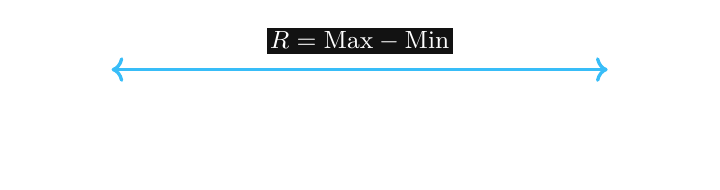
\begin{tikzpicture}[scale=1.05]
  \draw[base,->] (0,0) -- (8,0);
  \node[dot] at (1,0) {};
  \node[dot] at (7,0) {};
  \node[lab] at (1,-0.35) {Min};
  \node[lab] at (7,-0.35) {Max};
  \draw[new,<->] (1,0.55) -- (7,0.55);
  \node[lab, fill=pairbg, inner sep=1.2pt] at (4,0.9) {$R=\text{Max}-\text{Min}$};
\end{tikzpicture}
\end{StepDiagram}

\item \textbf{Mean (grouped):} using class midpoints $x_i$,
\[
\bar x=\frac{\sum f_i x_i}{\sum f_i}.
\]


\item \textbf{Variance (grouped, population):}


\[
\sigma^2=\frac{\sum f_i(x_i-\bar x)^2}{\sum f_i}
=\frac{\sum f_i x_i^2}{\sum f_i}-\bar x^{\,2}.
\]



\item \textbf{Standard deviation:}


\[
\sigma=\sqrt{\sigma^2}.
\]



\item \textbf{Coefficient of variation:}


\[
\mathrm{CV}=\frac{\sigma}{\bar x}\times 100\%.
\]



\end{itemize}

\end{QuickBox}

% ============================================================
% Q1
\begin{QAPair}{Question 1}
\textcolor{gold}{\bfseries Question:} What is dispersion? Write names and formulae of 3 measures of dispersion.
\tcblower
\textcolor{green}{\bfseries Answer:}\par

\textbf{Dispersion} means the \textbf{spread} or \textbf{variation} of data values around a central value (like mean). A small dispersion means data are close together; a large dispersion means data are more spread out.

\Step{1} \textbf{Range}
\[
R=\text{Max}-\text{Min}.
\]

\Step{2} \textbf{Mean Deviation (about mean)}
\[
\mathrm{MD}=\frac{\sum |x_i-\bar x|}{n}
\quad\text{or (grouped)}\quad
\mathrm{MD}=\frac{\sum f_i|x_i-\bar x|}{\sum f_i}.
\]

\Step{3} \textbf{Variance / Standard Deviation}
\[
\sigma^2=\frac{\sum (x_i-\bar x)^2}{n}
\quad\text{or (grouped)}\quad
\sigma^2=\frac{\sum f_i(x_i-\bar x)^2}{\sum f_i},
\qquad
\sigma=\sqrt{\sigma^2}.
\]
\end{QAPair}

% ============================================================
% Q2
\begin{QAPair}{Question 2}
\textcolor{gold}{\bfseries Question:} The energy consumption for a month is given below for Rabee's home.\\
\textbf{Units consumed:} $101\!-\!200,\;201\!-\!300,\;301\!-\!400,\;401\!-\!500,\;501\!-\!600,\;601\!-\!700$\\
\textbf{No. of months:} $2,\;1,\;3,\;1,\;3,\;2$\\
Find \textbf{Range} and \textbf{variance} of the energy consumption.
\tcblower
\textcolor{green}{\bfseries Answer:}\par

\Step{1} \textbf{Range}
\[
R=700-101=599.
\]
\EqDiagram{$\boxed{R=599\text{ units}}$}

\Step{2} \textbf{Midpoints} $x_i$ of each class:
\[
150.5,\;250.5,\;350.5,\;450.5,\;550.5,\;650.5
\]
and total months $N=\sum f=2+1+3+1+3+2=12$.

\Step{3} Compute $\bar x=\dfrac{\sum f x}{N}$ and $\sigma^2=\dfrac{\sum f x^2}{N}-\bar x^2$.

\begin{StepDiagram}
\StatTable{%
\begin{tabular}{|c|c|c|c|c|}
\hline
\textbf{Class} & $\boldsymbol{f}$ & $\boldsymbol{x}$ (mid) & $\boldsymbol{fx}$ & $\boldsymbol{f x^2}$\\
\hline
$101\!-\!200$ & 2 & 150.5 & 301.0 & 45{,}300.50\\
$201\!-\!300$ & 1 & 250.5 & 250.5 & 62{,}750.25\\
$301\!-\!400$ & 3 & 350.5 & 1{,}051.5 & 368{,}550.75\\
$401\!-\!500$ & 1 & 450.5 & 450.5 & 202{,}950.25\\
$501\!-\!600$ & 3 & 550.5 & 1{,}651.5 & 909{,}150.75\\
$601\!-\!700$ & 2 & 650.5 & 1{,}301.0 & 846{,}300.50\\
\hline
\textbf{Total} & \textbf{12} &  & $\sum fx=5{,}006$ & $\sum f x^2=2{,}435{,}003$\\
\hline
\end{tabular}}
\end{StepDiagram}

\Step{4} Mean:
\[
\bar x=\frac{5006}{12}=\frac{2503}{6}\approx 417.17.
\]

\Step{5} Variance:
\[
\sigma^2=\frac{2{,}435{,}003}{12}-\left(\frac{2503}{6}\right)^2
=\frac{260{,}000}{9}\approx 28{,}888.89.
\]

\[
\boxed{R=599\text{ units}\qquad \sigma^2\approx 28{,}888.89\text{ (units}^2\text{)}}
\]
\end{QAPair}

% ============================================================
% Q3
\begin{QAPair}{Question 3}
\textcolor{gold}{\bfseries Question:} Maria wants to analyze the water supply in her area, given in the data as shown.\\
\textbf{Water supply (gallons):} $501\!-\!700,\;701\!-\!900,\;901\!-\!1100,\;1101\!-\!1300$\\
\textbf{No. of hours:} $4,\;3,\;2,\;1$\\
Find: (i) mean supply, (ii) variance, (iii) SD, (iv) CV.
\tcblower
\textcolor{green}{\bfseries Answer:}\par

\Step{1} Midpoints $x_i$:
\[
600.5,\;800.5,\;1000.5,\;1200.5,\qquad N=\sum f=4+3+2+1=10.
\]

\begin{StepDiagram}
\StatTable{%
\begin{tabular}{|c|c|c|c|c|}
\hline
\textbf{Class} & $f$ & $x$ & $fx$ & $f x^2$\\
\hline
$501\!-\!700$ & 4 & 600.5 & 2{,}402.0 & 1{,}442{,}401.00\\
$701\!-\!900$ & 3 & 800.5 & 2{,}401.5 & 1{,}922{,}401.50\\
$901\!-\!1100$ & 2 & 1000.5 & 2{,}001.0 & 2{,}002{,}000.50\\
$1101\!-\!1300$ & 1 & 1200.5 & 1{,}200.5 & 1{,}441{,}200.25\\
\hline
\textbf{Total} & \textbf{10} &  & $\sum fx=8{,}005$ & $\sum f x^2=6{,}808{,}002.25$\\
\hline
\end{tabular}}
\end{StepDiagram}

\Step{2} Mean:
\[
\bar x=\frac{\sum fx}{N}=\frac{8005}{10}=800.5.
\]

\Step{3} Variance:
\[
\sigma^2=\frac{\sum f x^2}{N}-\bar x^2
=680{,}800.225-640{,}800.25=40{,}000.
\]

\Step{4} Standard deviation and CV:
\[
\sigma=\sqrt{40{,}000}=200,\qquad
\mathrm{CV}=\frac{200}{800.5}\times 100\%\approx 24.98\%.
\]

\[
\boxed{\bar x=800.5\text{ gal}\quad \sigma^2=40{,}000\quad \sigma=200\text{ gal}\quad \mathrm{CV}\approx 24.98\%}
\]
\end{QAPair}

% ============================================================
% Q4
\begin{QAPair}{Question 4}
\textcolor{gold}{\bfseries Question:} An organization wants to analyze salaries, grouped by department as shown: \\
Elementary: $40{,}000\!-\!60{,}000$ (10 employees),\\
Secondary: $60{,}000\!-\!80{,}000$ (12 employees),\\
Higher secondary: $80{,}000\!-\!100{,}000$ (8 employees).\\
Find the \textbf{range, variance, standard deviation} of the salaries across all departments. Also calculate \textbf{CV}.
\tcblower
\textcolor{green}{\bfseries Answer:}\par

\Step{1} \textbf{Range}
\[
R=100{,}000-40{,}000=60{,}000.
\]

\Step{2} Midpoints:
\[
50{,}000,\;70{,}000,\;90{,}000,\qquad N=10+12+8=30.
\]

\begin{StepDiagram}
\StatTable{%
\begin{tabular}{|c|c|c|c|c|}
\hline
\textbf{Salary range} & $f$ & $x$ & $fx$ & $f x^2$\\
\hline
$40{,}000\!-\!60{,}000$ & 10 & 50{,}000 & 500{,}000 & 25{,}000{,}000{,}000\\
$60{,}000\!-\!80{,}000$ & 12 & 70{,}000 & 840{,}000 & 58{,}800{,}000{,}000\\
$80{,}000\!-\!100{,}000$ & 8 & 90{,}000 & 720{,}000 & 64{,}800{,}000{,}000\\
\hline
\textbf{Total} & \textbf{30} &  & $\sum fx=2{,}060{,}000$ & $\sum f x^2=148{,}600{,}000{,}000$\\
\hline
\end{tabular}}
\end{StepDiagram}

\Step{3} Mean:
\[
\bar x=\frac{2{,}060{,}000}{30}=\frac{206{,}000}{3}\approx 68{,}666.67.
\]

\Step{4} Variance:
\[
\sigma^2=\frac{148{,}600{,}000{,}000}{30}-\left(\frac{206{,}000}{3}\right)^2
=\frac{2{,}144{,}000{,}000}{9}\approx 238{,}222{,}222.22.
\]

\Step{5} SD and CV:
\[
\sigma=\sqrt{\sigma^2}\approx 15{,}434.45,\qquad
\mathrm{CV}=\frac{15{,}434.45}{68{,}666.67}\times 100\%\approx 22.47\%.
\]

\[
\boxed{R=60{,}000\quad \sigma^2\approx 238{,}222{,}222.22\quad \sigma\approx 15{,}434.45\quad \mathrm{CV}\approx 22.47\%}
\]
\end{QAPair}

% ============================================================
% Q5
\begin{QAPair}{Question 5}
\textcolor{gold}{\bfseries Question:} A teacher wants to analyze the scores of students in different sections of class 10 as shown: \\
10 Mauve: $70\!-\!80$ (15 students),\;
10 teal: $60\!-\!70$ (12 students),\;
10 hazel: $50\!-\!60$ (10 students).\\
Find the \textbf{variance} and \textbf{standard deviation} of the grades of all sections.
\tcblower
\textcolor{green}{\bfseries Answer:}\par

\Step{1} Midpoints:
\[
75,\;65,\;55,\qquad N=15+12+10=37.
\]

\Step{2} Compute totals:
\[
\sum fx=15(75)+12(65)+10(55)=2{,}455,
\]
\[
\sum f x^2=15(75^2)+12(65^2)+10(55^2)=162{,}875.
\]

\Step{3} Mean:
\[
\bar x=\frac{2455}{37}\approx 66.35.
\]

\Step{4} Variance:
\[
\sigma^2=\frac{162{,}875}{37}-\left(\frac{2455}{37}\right)^2
=\frac{90{,}000}{1369}\approx 65.74.
\]

\Step{5} Standard deviation:
\[
\sigma=\sqrt{\frac{90{,}000}{1369}}=\frac{300}{37}\approx 8.11.
\]

\[
\boxed{\sigma^2\approx 65.74\qquad \sigma\approx 8.11}
\]
\end{QAPair}

% ============================================================
% Q6
\begin{QAPair}{Question 6}
\textcolor{gold}{\bfseries Question:} Mutahhir wants to analyze the purchases made by customers, grouped by age as shown: \\
Kids: $0\!-\!500$ (20 customers),\;
Juniors: $500\!-\!1000$ (30 customers),\;
Seniors: $1000\!-\!2000$ (25 customers).\\
Find the \textbf{range, variance} and \textbf{standard deviation} of the purchases across all age groups.
\tcblower
\textcolor{green}{\bfseries Answer:}\par

\Step{1} \textbf{Range}
\[
R=2000-0=2000.
\]

\Step{2} Midpoints:
\[
250,\;750,\;1500,\qquad N=20+30+25=75.
\]

\Step{3} Totals:
\[
\sum fx=20(250)+30(750)+25(1500)=65{,}000,
\]
\[
\sum f x^2=20(250^2)+30(750^2)+25(1500^2)=74{,}375{,}000.
\]

\Step{4} Mean (needed for variance):
\[
\bar x=\frac{65{,}000}{75}=\frac{2600}{3}\approx 866.67.
\]

\Step{5} Variance and SD:
\[
\sigma^2=\frac{74{,}375{,}000}{75}-\left(\frac{2600}{3}\right)^2
=\frac{2{,}165{,}000}{9}\approx 240{,}555.56,
\]
\[
\sigma=\sqrt{\sigma^2}\approx 490.46.
\]

\[
\boxed{R=2000\qquad \sigma^2\approx 240{,}555.56\qquad \sigma\approx 490.46}
\]
\end{QAPair}

% ============================================================
% Q7
\begin{QAPair}{Question 7}
\textcolor{gold}{\bfseries Question:} Namra wants to analyze blood pressure of patients in OT \& OPD grouped as shown.\\
\textbf{BP classes:} $100\!-\!110,\;110\!-\!120,\;120\!-\!130,\;130\!-\!140,\;140\!-\!150,\;150\!-\!160$\\
\textbf{Patients in OT (frequencies):} $3,8,6,7,4,2$\\
\textbf{Patients in OPD (frequencies):} $9,11,5,7,6,2$\\
Find the \textbf{Range, Mean, Variance, SD} of both datasets. Also find \textbf{CV} and comment on results.
\tcblower
\textcolor{green}{\bfseries Answer:}\par

\Step{1} Range (same classes for both):
\[
R=160-100=60.
\]

\Step{2} Midpoints:
\[
105,\;115,\;125,\;135,\;145,\;155.
\]

\Step{3} \textbf{OT calculations} ($f=\{3,8,6,7,4,2\}$, $N=30$)

\[
\bar x_{\text{OT}}=\frac{\sum fx}{N}=\frac{382}{3}\approx 127.33,
\]
\[
\sigma^2_{\text{OT}}=\frac{\sum f x^2}{N}-\bar x_{\text{OT}}^{\,2}
=\frac{1781}{9}\approx 197.89,
\qquad
\sigma_{\text{OT}}=\sqrt{\sigma^2_{\text{OT}}}\approx 14.07,
\]
\[
\mathrm{CV}_{\text{OT}}=\frac{14.07}{127.33}\times 100\%\approx 11.05\%.
\]

\Step{4} \textbf{OPD calculations} ($f=\{9,11,5,7,6,2\}$, $N=40$)

\[
\bar x_{\text{OPD}}=\frac{\sum fx}{N}=124.00,
\]
\[
\sigma^2_{\text{OPD}}=\frac{\sum f x^2}{N}-\bar x_{\text{OPD}}^{\,2}
=239.00,
\qquad
\sigma_{\text{OPD}}=\sqrt{239}\approx 15.46,
\]
\[
\mathrm{CV}_{\text{OPD}}=\frac{15.46}{124}\times 100\%\approx 12.47\%.
\]

\Step{5} \textbf{Comment:} OPD has \textbf{higher variance and CV}, so OPD blood pressures are \textbf{more spread out} (more variability) than OT.

\[
\boxed{
\begin{aligned}
&\text{Range}=60 \text{ (both)}\\
&\text{OT: }\bar x\approx 127.33,\;\sigma^2\approx 197.89,\;\sigma\approx 14.07,\;\mathrm{CV}\approx 11.05\%\\
&\text{OPD: }\bar x=124.00,\;\sigma^2=239.00,\;\sigma\approx 15.46,\;\mathrm{CV}\approx 12.47\%
\end{aligned}}
\]
\end{QAPair}

% ============================================================
% Q8
\begin{QAPair}{Question 8}
\textcolor{gold}{\bfseries Question:} Khola wants to forecast the temperature for the next week for Jhelum and Indiana.\\
\textbf{Jhelum (F):} $96\!-\!100,\,101\!-\!105,\,106\!-\!110,\,111\!-\!115$ with days $2,3,1,1$.\\
\textbf{Indiana (F):} $51\!-\!60,\,61\!-\!70,\,71\!-\!80,\,81\!-\!90$ with days $3,1,2,1$.\\
Find (i) \textbf{Mean} of both datasets, (ii) \textbf{Variance} of both datasets. Also comment on possible predictions.
\tcblower
\textcolor{green}{\bfseries Answer:}\par

\Step{1} \textbf{Jhelum:} midpoints $98,103,108,113$, $N=7$.
\[
\bar x_J=\frac{726}{7}\approx 103.71,
\qquad
\sigma_J^2=\frac{1200}{49}\approx 24.49.
\]

\Step{2} \textbf{Indiana:} midpoints $55.5,65.5,75.5,85.5$, $N=7$.
\[
\bar x_I=\frac{937}{14}\approx 66.93,
\qquad
\sigma_I^2=\frac{6200}{49}\approx 126.53.
\]

\Step{3} \textbf{Comment (prediction idea):}
Variance measures spread/uncertainty. Since Indiana has a \textbf{much larger variance}, its temperatures are \textbf{more variable}, so predictions for next week are \textbf{less certain}. Jhelum has smaller variance, so temperatures are \textbf{more stable} and easier to predict.

\[
\boxed{
\text{Jhelum: }\bar x\approx 103.71,\;\sigma^2\approx 24.49
\qquad
\text{Indiana: }\bar x\approx 66.93,\;\sigma^2\approx 126.53}
\]
\end{QAPair}

\end{document}
